% =====================================================================
%  CasaMotion — Descriptif succinct du projet (livrable 3 pages)
%  Compilation : pdflatex livrable_3pages.tex  (2 passes)
%  Charte graphique reprise du deck CasaMotion (cyan -> bleu -> violet)
% =====================================================================
\documentclass[10pt,a4paper]{article}

\usepackage[T1]{fontenc}
\usepackage[utf8]{inputenc}
\usepackage[french]{babel}
\usepackage{lmodern}
\usepackage{amsmath,amssymb}
\usepackage[a4paper,margin=1.5cm,top=1.3cm,bottom=1.3cm]{geometry}
\usepackage[table]{xcolor}
\usepackage{titlesec}
\usepackage{enumitem}
\usepackage{booktabs}
\usepackage{array}
\usepackage{multicol}
\usepackage{tcolorbox}
\usepackage{microtype}
\usepackage[hidelinks]{hyperref}
\usepackage{tikz}
\usetikzlibrary{shadows}
\tcbuselibrary{skins,breakable}
\graphicspath{{../presentation/assets/}{./}}

% ---- Charte CasaMotion -------------------------------------------------
\definecolor{casacyan}{HTML}{15C2E6}
\definecolor{casablue}{HTML}{2D6BFF}
\definecolor{casaviolet}{HTML}{7B3DF5}
\definecolor{casanavy}{HTML}{0A1330}
\definecolor{casaink}{HTML}{26335C}
\definecolor{casamuted}{HTML}{5E6C8E}
\definecolor{casapanel}{HTML}{F4F7FD}
\definecolor{casaline}{HTML}{D9E1F2}
\definecolor{casaok}{HTML}{16A36A}
\definecolor{casawarn}{HTML}{D98A16}

% ---- Réglages typographiques compacts ----------------------------------
\setlength{\parindent}{0pt}
\setlength{\parskip}{2pt}
\linespread{0.99}
\setlist[itemize]{leftmargin=1.05em,itemsep=1pt,topsep=2pt,parsep=0pt}
\setlist[enumerate]{leftmargin=1.4em,itemsep=1pt,topsep=2pt,parsep=0pt}
\pagestyle{empty}

% ---- Titres de section avec carré dégradé ------------------------------
\titleformat{\section}
  {\normalfont\large\bfseries\color{casanavy}}
  {\textcolor{casablue}{\rule[0.12ex]{0.9ex}{0.9ex}}\,}{0.5em}{}
  [{\color{casaline}\titlerule[1pt]}]
\titlespacing*{\section}{0pt}{6pt}{3pt}

\titleformat{\subsection}
  {\normalfont\normalsize\bfseries\color{casablue}}{}{0em}{}
\titlespacing*{\subsection}{0pt}{4pt}{1pt}

% ---- Boîte "encadré" réutilisable --------------------------------------
\newtcolorbox{casabox}[1][casablue]{
  enhanced, breakable, sharp corners,
  colback=casapanel, colframe=#1,
  boxrule=0pt, leftrule=2.4pt,
  left=7pt, right=7pt, top=4pt, bottom=4pt,
  fonttitle=\bfseries\color{casanavy}
}

% ---- Cadre figure moderne (coins arrondis) -----------------------------
\newtcolorbox{figbox}{
  enhanced, arc=3pt, colback=white, colframe=casaline,
  boxrule=0.6pt, left=3pt, right=3pt, top=3pt, bottom=3pt,
  halign=center, drop shadow=casaline
}
\newcommand{\figcap}[1]{{\centering\vspace{1pt}\scriptsize\color{casamuted}\textit{#1}\par}}

\newcommand{\kw}[1]{\textcolor{casablue}{\textbf{#1}}}
\newcommand{\chip}[1]{\tcbox[on line,boxsep=1pt,left=3pt,right=3pt,top=1pt,
  bottom=1pt,colback=casapanel,colframe=casaline,boxrule=0.4pt,
  fontupper=\footnotesize\ttfamily\color{casaink}]{#1}}

% ---- Barre dégradée signature (cyan -> bleu -> violet) ------------------
\newcommand{\gradientbar}[1][3.2pt]{%
  \noindent\begin{tikzpicture}
    \shade[left color=casacyan,middle color=casablue,right color=casaviolet]
      (0,0) rectangle (\linewidth,#1);
  \end{tikzpicture}}

\begin{document}

% =====================================================================
%  EN-TÊTE (clair, avec logo CasaMotion)
% =====================================================================
\noindent
\begin{minipage}[b]{0.66\linewidth}
  
\includegraphics[height=14mm]{logo-nav-gradient.png}
\end{minipage}\hfill
\begin{minipage}[b]{0.32\linewidth}
  \raggedleft
  {\footnotesize\bfseries\color{casanavy}Descriptif succinct du projet}\\[1pt]
  {\scriptsize\color{casamuted}\ttfamily Intelligence de mobilité urbaine\\ en temps réel}\\[3pt]
  {\scriptsize\color{casaink}\textbf{\'Equipe :} Mohamed Amine El Abidi\\ \& Rida Aderkane}
\end{minipage}

\vspace{5pt}
\gradientbar

\vspace{4pt}
{\footnotesize\color{casaink} Plateforme de données streaming pour \textbf{Casablanca} :
matching rider/véhicule, prévision de la demande et observabilité à l'échelle de la
ville. \textcolor{casamuted}{Méthodologies, réalisations et conclusions ; livrable
accompagné du code source et d'extraits de données.}}\\[1pt]
{\scriptsize\color{casamuted}\ttfamily Architecture Kappa / 16 conteneurs Docker /
Kafka / Flink / Spark / Cassandra / MinIO / FastAPI / Grafana}\\[2pt]
{\scriptsize\color{casamuted}\ttfamily Code source :\ }%
\href{https://github.com/mohamedamineelabidi/CasaMotion}{\scriptsize\color{casablue}\ttfamily github.com/mohamedamineelabidi/CasaMotion}

% =====================================================================
%  1. CONTEXTE & OBJECTIFS
% =====================================================================
\section{Contexte \& objectifs}
\begin{multicols}{2}
\kw{Problème.} Casablanca (\textasciitilde 4\,M d'habitants) ne dispose
d'\textbf{aucune couche de données partagée} pour sa mobilité : grands/petits
taxis et minibus circulent sans GPS, sans réservation ni horaire. Conséquences :
chauffeurs à vide, attente des usagers, absence d'interopérabilité
(rail/BRT/taxi), paiement en espèces sans historique exploitable. \emph{Le
véritable manque est une couche de données reliant l'offre à la demande, pas un
manque de véhicules.}

\columnbreak

\kw{Objectifs (cahier des charges).}
\begin{itemize}
  \item Matching \textbf{rider–véhicule} en moins de 5 s.
  \item Prévision de la \textbf{demande par zone} à 30 min.
  \item \textbf{Visibilité ville} : heatmaps, KPI, zones sous-desservies.
  \item \textbf{Planification} pilotée par la donnée.
\end{itemize}
Chaîne attendue : ingestion temps réel · traitement \emph{event-time} · base de
service · ML batch · dashboards · API sécurisée.
\end{multicols}

% =====================================================================
%  2. ARCHITECTURE & CHOIX TECHNIQUES
% =====================================================================
\section{Architecture \& choix techniques}
\begin{multicols}{2}
\kw{Pipeline (Kappa).} \chip{Producteurs} $\rightarrow$ \chip{Kafka (KRaft)}
$\rightarrow$ \chip{3 jobs Flink} $\rightarrow$ \chip{Cassandra} $\rightarrow$
\chip{Grafana / FastAPI}. \textbf{Kafka est la source de vérité unique et
rejouable} ; MinIO est le \emph{data lake} S3 ; Spark est strictement
\textbf{hors-ligne} (batch + ML). C'est une architecture \textbf{Kappa} (une
seule couche de traitement), et non Lambda.

\columnbreak

\footnotesize
\begin{tabular}{@{}>{\bfseries}l l@{}}
\toprule
\rowcolor{casapanel}\color{casanavy}Choix & \color{casanavy}Justification \\
\midrule
Kappa & 1 couche ; Kafka rejouable \\
Kafka KRaft & sans ZooKeeper, bascule + rapide \\
Flink & fenêtres \emph{event-time}, latence < s \\
Cassandra & écriture optimisée, TTL natif \\
MinIO & API S3 (Spark/Flink/Connect) \\
H3 res-9 & lookup zone en O(1) \\
\bottomrule
\end{tabular}
\end{multicols}

\vspace{3pt}
\begin{figbox}
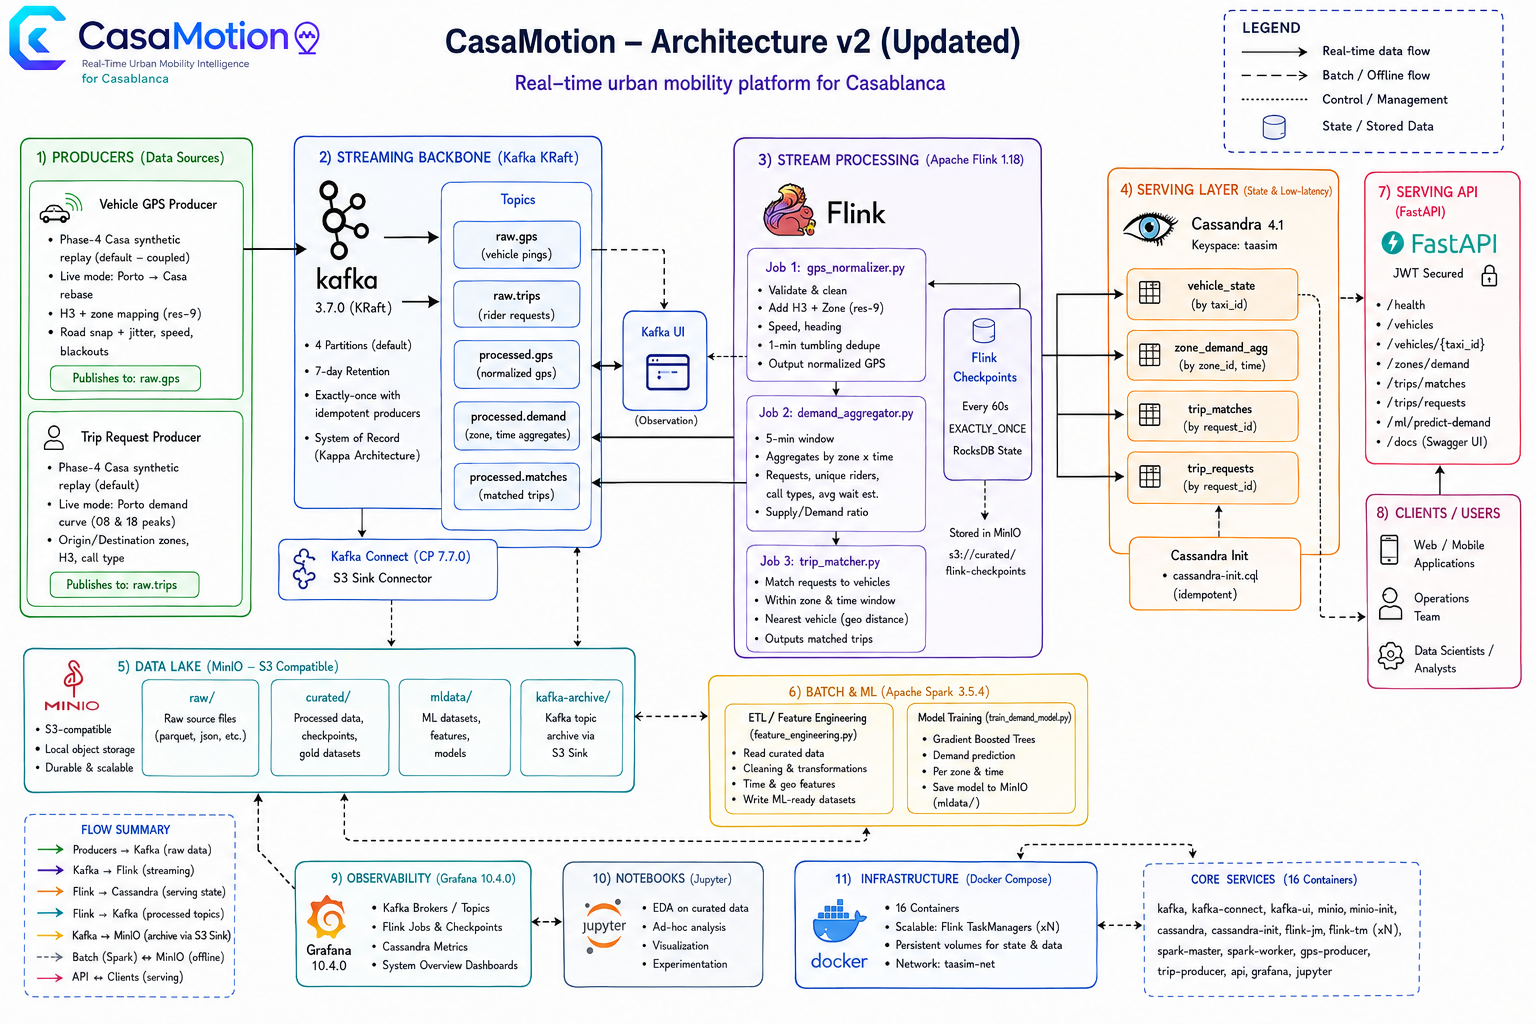
\includegraphics[width=\linewidth]{architecturev2.png}
\end{figbox}
\figcap{Figure 1 — Architecture de bout en bout : producteurs $\rightarrow$ Kafka (KRaft)
$\rightarrow$ 3 jobs Flink $\rightarrow$ Cassandra ; data lake MinIO, batch Spark/ML hors-ligne, API FastAPI
et observabilité Grafana.}

% =====================================================================
%  3. MÉTHODOLOGIE — ÉTAPES DU PROJET
% =====================================================================
\section{Méthodologie — étapes du projet}

\subsection{Semaine 1 — Fondations \& géographie}
\begin{itemize}
  \item \kw{Stack Docker} (Kafka, MinIO, Cassandra, Flink, Spark, Grafana,
  Jupyter) ; datasets \textbf{Porto} (1,8 GiB) + \textbf{NYC TLC} chargés dans MinIO.
  \item \kw{Découpage en 16 zones} : 9 polygones administratifs OSM + 7 cellules
  de Voronoï (banlieues nord), nettoyés des chevauchements et bords maritimes.
  \item \kw{Score d'activité A–E} par zone :
  $\text{score}_z = 0{,}40\,\rho + 0{,}30\,c + 0{,}20\,d + 0{,}10\,t$
  (densité de population HCP\,2024, commerce et diversité POI via Glovo, hubs de
  transit OSM), normalisé puis découpé en quantiles.
  \item \kw{Lookup H3 res-9} pré-calculé (\chip{h3\_zone\_lookup.json}) :
  affectation de zone en \textbf{O(1)} au lieu d'un \emph{point-in-polygon}.
  \item \kw{Warping Porto $\rightarrow$ Casablanca} : transformation affine
  bbox, ancrage au centroïde + jitter, puis routage \textbf{OSRM} sur le réseau
  routier réel de Casablanca.
\end{itemize}

\subsection{Semaine 2 — Couche de stockage}
\begin{itemize}
  \item \kw{Kafka Connect (S3 Sink)} : archivage \chip{raw.gps} / \chip{raw.trips}
  vers MinIO, partitionné par heure.
  \item \kw{Schéma Cassandra} conçu \textbf{autour des requêtes} : 3 tables avec
  TTL ; partition \chip{date\_bucket} pour borner la taille. \textbf{ADR v1}
  documentant chaque décision.
\end{itemize}

\subsection{Semaine 3 — Traitement temps réel (PyFlink)}
\begin{itemize}
  \item \kw{Job 1 — Normalizer GPS} : validation, déduplication, zone H3,
  \textbf{anonymisation} (centroïde + jitter haché) $\rightarrow$ \chip{vehicle\_positions}.
  \item \kw{Job 2 — Agrégateur de demande} : fenêtres glissantes 30 s par zone,
  ratio offre/demande $\rightarrow$ \chip{demand\_zones}.
  \item \kw{Job 3 — Matcher} : \emph{keyBy} zone, pool de véhicules en MapState,
  \emph{fan-out} vers zones adjacentes + déduplication $\rightarrow$ \chip{trips}.
  \item \kw{Garanties} : checkpoints RocksDB \textbf{EXACTLY\_ONCE} (60 s) vers
  MinIO ; \emph{watermarks} (3 min / 10 s + idleness) pour les événements tardifs.
\end{itemize}

\subsection{Semaine 5 — ETL batch (Spark)}
\begin{itemize}
  \item \kw{Porto} : 1\,710\,670 $\rightarrow$ 1\,660\,794 trajets valides
  $\rightarrow$ Parquet curated (43 MiB).
  \item \kw{NYC TLC} : 9,38\,M $\rightarrow$ 8,81\,M $\rightarrow$ \textbf{192\,K
  lignes de demande}. \textbf{Règle Kappa : NYC reste batch-only, ne transite
  jamais par Kafka et n'entraîne pas le modèle.}
\end{itemize}

\subsection{Semaine 6 — Machine Learning + API}
\begin{itemize}
  \item \kw{Feature engineering} : matrice de \textbf{183\,981 lignes} ; cible =
  trajets par zone par créneau de 30 min.
  \item \kw{Anti-fuite (leakage)} : suppression de \chip{supply} /
  \chip{supply\_demand\_ratio} (issus du même créneau que la cible) ; conservation
  des seules variables rétrospectives (lags 1\,j / 7\,j, moyenne mobile 7\,j).
  \item \kw{Split temporel} (et non aléatoire) au \chip{2014-05-01} :
  entraînement 151\,911 / test 32\,070.
  \item \kw{Modèle} : Spark MLlib \chip{GBTRegressor} (maxDepth=5, maxIter=50),
  \emph{pipeline} StringIndexer $\rightarrow$ VectorAssembler $\rightarrow$ GBT.
\end{itemize}

% =====================================================================
%  3bis. DONNÉES & ARTEFACTS (EXTRAITS)
% =====================================================================
\section{Données \& artefacts (extraits fournis)}
\footnotesize
\begin{tabular}{@{}>{\ttfamily}l l l@{}}
\toprule
\rowcolor{casapanel}\color{casanavy}\normalfont Artefact & \color{casanavy}Rôle & \color{casanavy}Volume / format \\
\midrule
data/train.csv            & Source Porto (polylines GPS, donneur)      & 1,71\,M trajets · CSV \\
data/nyc-tlc/*.parquet    & Motifs de demande NYC (batch-only)         & 9,38\,M lignes · Parquet \\
data/zone\_mapping\_v4.csv  & 16 zones + score A--E + centroïdes         & 16 lignes · CSV \\
data/h3\_zone\_lookup.json  & Index H3 res-9 $\rightarrow$ zone (O(1))   & JSON \\
curated/trips/            & Trajets nettoyés (sortie Spark ETL)        & 43 MiB · Parquet \\
mldata/features/          & Matrice d'apprentissage (anti-leakage)     & 183\,981 lignes · Parquet \\
mldata/models/demand\_v1/  & Pipeline GBT entraîné (StringIndexer+GBT)  & Spark MLlib \\
\bottomrule
\end{tabular}
\normalsize
\vspace{2pt}

{\footnotesize\color{casamuted} Flux de bout en bout :}\;
\chip{raw.gps / raw.trips} $\rightarrow$ \chip{Flink (3 jobs)} $\rightarrow$
\chip{vehicle\_positions · demand\_zones · trips} (Cassandra) ; en parallèle
\chip{Kafka Connect} archive vers MinIO et \chip{Spark} produit \chip{curated/}
puis \chip{mldata/} consommé par \chip{FastAPI}.

% =====================================================================
%  4. RÉALISATIONS & RÉSULTATS
% =====================================================================
\section{Réalisations \& résultats mesurés}
\begin{multicols}{2}
\footnotesize
\begin{tabular}{@{}l c c@{}}
\toprule
\rowcolor{casapanel}\color{casanavy}Métrique & \color{casanavy}Cible & \color{casanavy}Mesuré \\
\midrule
Matching (P95)        & < 5 s   & \textbf{\textasciitilde 1,2 s}\,\textcolor{casaok}{\checkmark} \\
Fraîcheur GPS         & < 15 s  & \textbf{\textasciitilde 4 s}\,\textcolor{casaok}{\checkmark} \\
MAJ demande           & 30 s    & 30 s glissant\,\textcolor{casaok}{\checkmark} \\
ETL Porto (1,7\,M)    & < 5 min & 43 MiB Parquet\,\textcolor{casaok}{\checkmark} \\
Checkpoints Flink     & 60 s    & 25 conséc., 0 échec\,\textcolor{casaok}{\checkmark} \\
Charge API forecast   & <500 ms & test à venir\,\textcolor{casawarn}{$\circ$} \\
\bottomrule
\end{tabular}

\columnbreak

\kw{Modèle de prévision (GBT) vs baseline naïve (lag 7\,j) :}
\footnotesize
\begin{tabular}{@{}l c c@{}}
\toprule
\rowcolor{casapanel}\color{casanavy}Métrique & \color{casanavy}GBT & \color{casanavy}Naïf \\
\midrule
RMSE & \textbf{3,71} & 6,84 \\
MAE  & \textbf{2,11} & — \\
R\textsuperscript{2} & \textbf{0,75} & — \\
\midrule
\multicolumn{3}{@{}l}{\textbf{Amélioration RMSE : \textcolor{casablue}{$-45{,}8\%$}}}\\
\multicolumn{3}{@{}l}{\scriptsize Battu \textbf{globalement et sur les 16 zones}.}\\
\bottomrule
\end{tabular}
\end{multicols}

\vspace{2pt}
\begin{casabox}[casacyan]
\kw{Validation pilotée par la preuve.} \emph{Healthcheck} démo (16 vérifications :
conteneurs, jobs Flink RUNNING, fraîcheur des tables) ; tests de réalisme du
mouvement (8/8 distincts, 139/139 en mouvement, 200/200 < 100 m, 80/80 dans la
bbox) ; test d'événements tardifs / \emph{watermark} ; validation ML (split
temporel, table de comparaison à la baseline par zone).
\end{casabox}

% =====================================================================
%  5. CONCLUSIONS & PERSPECTIVES
% =====================================================================
\section{Conclusions \& perspectives}
\begin{multicols}{2}
\kw{Conclusions.}
\begin{itemize}
  \item Plateforme \textbf{temps réel de bout en bout} et reproductible
  (\chip{docker compose up -d}, 16 conteneurs) couvrant ingestion, traitement
  \emph{event-time}, service, ML batch et observabilité.
  \item Cibles de performance \textbf{atteintes ou dépassées} ; modèle ML
  \textbf{supérieur à la baseline} sur toutes les zones.
  \item \textbf{Confidentialité \emph{by design}} : les coordonnées brutes ne sont
  jamais persistées (centroïde + jitter).
\end{itemize}

\columnbreak

\kw{Limites assumées (honnêteté méthodologique).}
\begin{itemize}
  \item Données \textbf{donneuses} : mouvement réel de Porto + motifs de demande
  NYC, ré-ancrés via HCP\,2024 + Glovo (pas de jeu de données taxi Casablanca ouvert).
  \item 7 des 16 zones sont des \textbf{cellules de Voronoï} (échafaudage
  d'agrégation), non des arrondissements officiels.
  \item L'API sert par défaut une \textbf{heuristique} ; le modèle GBT Spark se
  charge en option (\chip{PYSPARK\_ENABLED=1}).
\end{itemize}

\kw{Perspectives (S7–S8).} Durcissement sécurité (rotation JWT, TLS, SASL/ACL
Kafka) ; tests d'intégration CI (P95 < 5 s) ; test de charge Locust ; démo de
reprise sur checkpoint.
\end{multicols}

\vspace{5pt}
\begin{figbox}
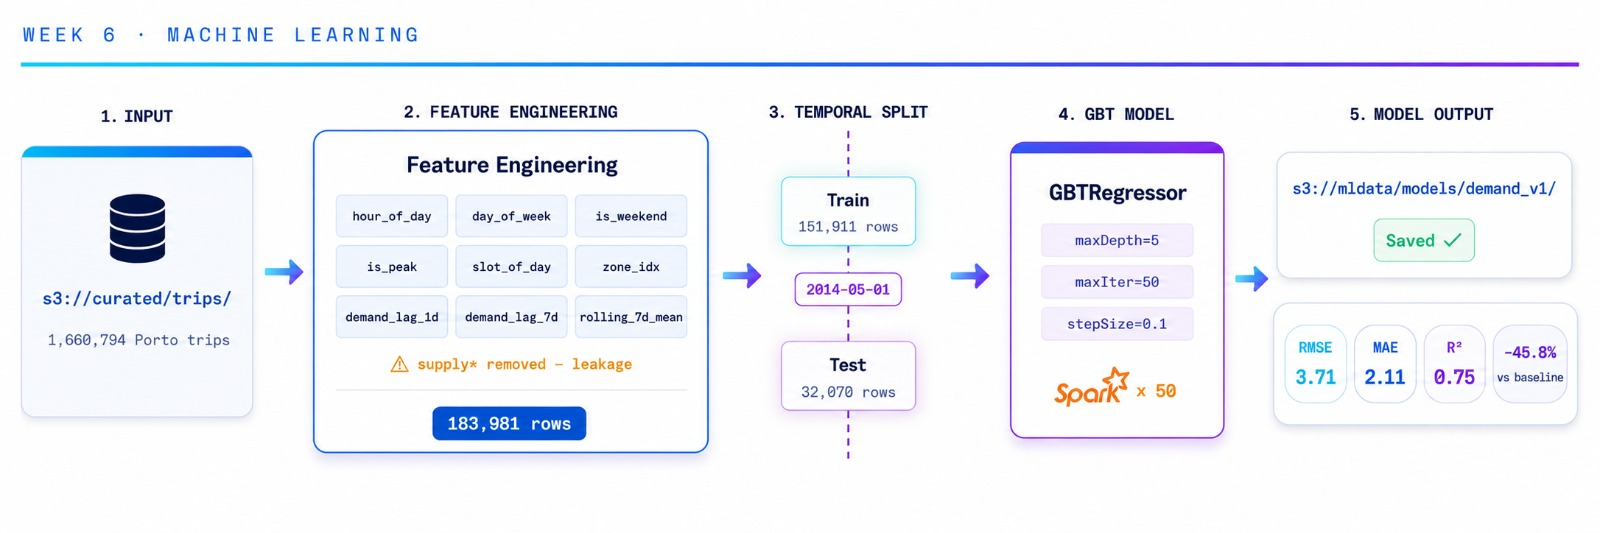
\includegraphics[width=\linewidth]{MLARCHITECTURE.png}
\end{figbox}
\figcap{Figure 2 — Pipeline d'apprentissage (Semaine 6) : trajets curated $\rightarrow$ feature
engineering anti-fuite (183\,981 lignes) $\rightarrow$ split temporel (2014-05-01) $\rightarrow$ GBTRegressor
$\rightarrow$ modèle servi (RMSE 3,71 ; $-45{,}8\%$ vs baseline).}

\vspace{6pt}
\begin{center}
\begin{minipage}{0.60\linewidth}
\begin{figbox}
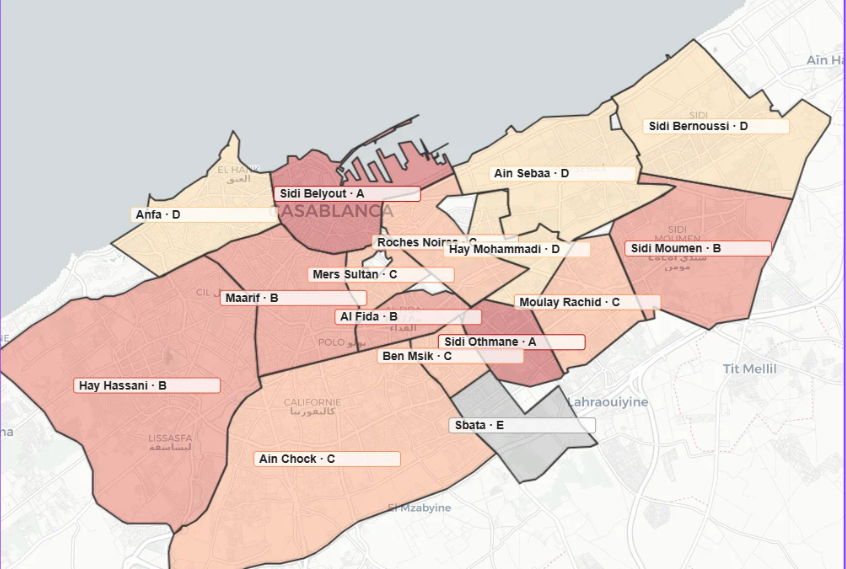
\includegraphics[width=\linewidth]{arrondissementcasabbox.png}
\end{figbox}
\figcap{Figure 3 — Découpage de Casablanca en 16 zones (9 arrondissements OSM
+ 7 cellules de Voronoï) borné par la bbox de la ville.}
\end{minipage}
\end{center}

\vspace{3pt}
\gradientbar[2pt]
\vspace{2pt}
\begin{center}
{\scriptsize\color{casamuted}\ttfamily CasaMotion -- livrable de synthese
~/~ Code source + extraits de donnees fournis separement
~/~ Architecture Kappa, 16 conteneurs, ML GBT}
\end{center}

\end{document}
